\ofsubsection{Chocobo}
%

\ofquote{"Não há maneira errada de se amar uma Chocobo."\\}{Noctis}\\\\
%
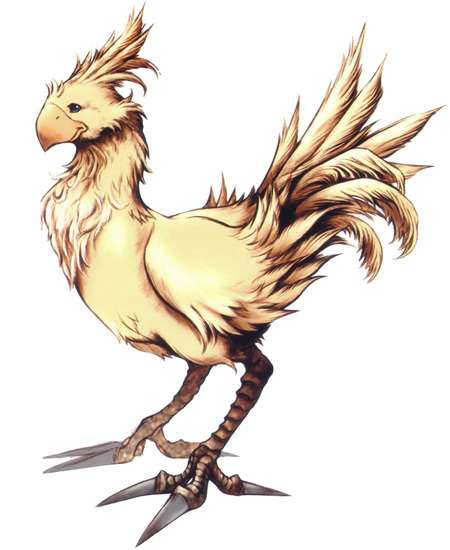
\includegraphics[width=0.95\columnwidth]{./art/chocobo/chocobo.jpg}
%
\\\\
%
%
\accf{Chocobos} são criaturas aviárias grandes e incapazes de voar, com penas amarelas e um longo pescoço. Elas são muito inteligentes e até entendem as línguas humanoides em certa medida.
Portanto, elas são com frequência domesticadas e usadas como montarias, parecido com os cavalos, e as alugar é um negócio lucrativo para fazendeiros.
Embora o preço possa flutuar, o grupo geralmente pode alugar uma delas por cerca de 10G por dia.
Em casos raros, fazendeiros também as vendem a preços exorbitantes, a partir de 3.000G.
O grupo também pode tentar capturar aquelas que vagam pela natureza, elas são normalmente encontradas em florestas ou pastagens selvagens.
Tais Chocobos comumente são hostis e só entram em combate ao se sentirem ameaçadas.
Ao receber qualquer dano, uma Chocobo selvagem realiza um teste de DF~7 e se falhar, fica assustada e foge o mais rápido que puder.
Um personagem pode ganhar a confiança delas ao usar sua ação para as alimentar com sua comida favorita, as \accf{Verduras Gysahl}.
Neste caso, o jogador realiza um teste de DF~6 + nível da Chocobo e se for bem sucedido, ela se juntará ao grupo e seguirá seus comandos a partir de então.
%
\ofpar
%
%\ofquote{"Fat Chocobo? You're rude! Here it's the bird of gods!"}{Dwarf}\\\\
%
Por serem criaturas aviárias, as Chocobos põem ovos.
Contudo, eles crescem surpreendentemente rápido: um ovo choca em algumas semanas após ser posto e depois de um mês, a maioria das Chocobos estão tão grandes quanto seus criadores.
Elas normalmente procriam em estábulos, onde são mantidas aquecidas e a salvo. Também podem ser de diferentes tipos, o que é determinado pela cor de suas penas.
A mais comum é a amarela, outros tipos são bem raras em comparação.
O tipo da Chocobo depende de seus progenitores e a tabela seguinte mostra o resultado de pares diferentes.
Em todo caso não listado, uma Chocobo tem o tipo de seus pais se eles forem ambos do mesmo tipo ou se ela for amarela.\\\\
%
\oftable{p{0.37\columnwidth} p{0.37\columnwidth} p{0.3\columnwidth}}
{\accf{Genitor 1} & \accf{Genitor 2} & \accf{Cria}} {
Amarela 	& Azul   & Verde \\
Amarela 	& Vermelha    & Verde \\
Azul 	& Verde  & Vermelha \\
Red 	& Verde  & Azul \\
Azul 	& Azul   & Branca \\
Vermelha 	& Vermelha    & Preta \\
Preta 	& Branca  & Dourada\\
}
%
\vfill
%
Este conhecimento está disponível a muitos criadores experientes de Chocobos ou em livros sobre o assunto.
O grupo pode tentar criar algumas dos tipos raros, as quais com frequência vêm com habilidades especiais.
Os detalhes sobre os diferentes tipos de Chocobos são mostrados ao fim dessa subseção.
Em alguns casos o tipo de uma Chocobo recém nascida pode não atender à tabela acima.
Sempre que alguma nova nasce, faça um teste de DF~11 e se bem sucedido, seu tipo é determinado imediatamente da seguinte maneira:
role 2d, ela será Branca se 2-3, Azul se 4-5, Amarela se 6-8, vermelha se 9-10 ou Preta se 11-12.
%
%\ofpar
%
Criar uma Chocobo não é uma tarefa simples, ela necessita de bastante cuidado e atenção. Em retorno, ela pode ajudar o grupo em várias situações através de suas capacidades únicas, que melhoram ao longo da aventura.
Assim sendo, níveis a mais funcionam um pouco diferente para elas.
Primeiro, uma Chocobo pode somente aprender um conjunto predeterminado de habilidades a depender de seu tipo.
Segundo, aumentos de atributos a cada nível a mais também funcionam diferente: o PV e PM máximo delas aumentam em +5 para cada nível a mais.
Além disso, seu dono pode gastar 3 pontos extras para melhorar ainda mais os atributos da Chocobo se desejar.
A tabela abaixo mostra quantos pontos é preciso gastar para diferentes bônus de atributo. Uma diferença a se notar se comparado aos personagens jogadores é de que as Chocobos possuem um atributo adicional \accf{Fôlego}, o qual determina sua afinidade a viagens de longa distância.
%
\ofpar
%
\oftable{p{0.5\columnwidth} p{0.3\columnwidth}} 
{\accf{Bônus de atributo} & \accf{Pontos}} {
  Max. PV +5 	& 1 \ofrow
  Max. PM +5 	& 1 \ofrow
  FOR +1 		& 1 \ofrow
  DEF +1 		& 1 \ofrow
  MAG +1 		& 1 \ofrow
  RES +1 		& 1 \ofrow
  FOL +1 		& 2 \ofrow
  DANO +1d 		& 3 \ofrow
  AGI +1 		& 3 \ofrow
}
%
\clearpage
%
%\ofquote{"Man... Chocobo, we just can’t get a break, can we?"\\}{Sazh}\\\\
\ofquote{"Meu cabelo NÃO parece como a bunda de uma Chocobo!"\\}{Prompto}\\\\
%
Os personagens podem montar em Chocobos para experienciar uma viagem rápida e confortável. Montar as que são domesticadas é simples, mas um cavaleiro experiente pode se sobressair em situações complicadas.
Elas podem carregar uma quantidade considerável de peso sem serem afetadas.
No entanto, as Chocobos se cansam depois de uma viagem prolongada e ininterrupta.
Elas podem andar uma quantidade de horas igual ao seu atributo Fôlego antes de precisarem de uma pausa.
Este tempo é a metade se a carga total por ela carregada exceder significativamente o equivalente a dois humanos.
Mesmo assim as Chocobos normalmente seguem as ordens de seus donos, elas podem se recusar a avançar sempre que se sentirem bem assustadas ou surpreendidas.
Também podem ser combatentes muito capazes e, portanto, adições cruciais às linhas para o grupo, lutando junto a eles, cujo caso elas são tratadas como qualquer outro combatente aliado participante.
Uma Chocobo é controlada pelo jogador cujo personagem é o seu dono e obedece a seus comandos.
Por outro lado, os personagens também podem decidir continuar montados durante o combate. Se isso acontecer, a Chocobo e seu dono sempre agirão juntos, sendo que somente ela lida com a movimentação.
Sempre que o cavaleiro ataca um inimigo pequeno ou médio enquanto montado, o alvo tem Desvantagem no teste de evasão.
Contudo, quando uma Chocobo sofre dano enquanto carregando seu cavaleiro, ela tem que realizar um teste de DF~12 - FOR. Se falhar, o cavaleiro é lançado ao chão e fica Imóvel por 1 rodada.
%
\vfill
%
\ofmonster{Chocobo amarela}{1}{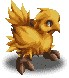
\includegraphics[width=0.23\columnwidth]{./art/chocobo/chocyellow.jpg}}
{
	PV: & \hfill 19 & PM: & \hfill 17\\
	FOR: & \hfill 1 & DEF: & \hfill 0 \\
	MAG: & \hfill 1 & RES: & \hfill 0 \\
	AGI: & \hfill 2 & FOL: & \hfill 2 \\
}
{\accf{Bico}: 1d Dano}
{
	\mspell{Cura (Nível 1)}{4}{0r}{Único}{3u}{O alvo recupera 2d de PV.}{\accf{Nível 1}}		
	\mspell{Esuna (Nível 3)}{6}{0r}{Único}{5u}{Remova todos os Estados de Efeito, exceto KO.}{\accf{Nível 3}}	
	\mtech{Enfurecer (Nível 6)}{10}{0r}{Único}{5u}{O alvo realiza um teste de DF~8 e se falhar, tem que se mover em direção a você no seu próximo turno e, se possível, atacá-lo.}{\accf{Nível 6}}	
	\mtech{Chocobo gorda (Nível 9)}{16}{1r}{1u}{5u}{Todos na área de efeito sofrem 6d de dano e ficam Imóveis por 1 rodada.}{\accf{Nível 9}\immobile}	
	\mpassive{Choco-planar}{Você pode planar devagar até o chão de alturas até 30u sem sofrer danos.}
}
%
\newpage
%
\ofquote{"Sabe, tudo que eu queria fazer é montar numa Chocobo. Mais rápido que o vento!"}{Clasko}\vfill
%
\ofmonster{Chocobo vermelha}{1}{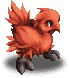
\includegraphics[width=0.23\columnwidth]{./art/chocobo/chocred.jpg}}
{
	PV: & \hfill 21 & PM: & \hfill 13\\
	FOR: & \hfill 2 & DEF: & \hfill 1 \\
	MAG: & \hfill 0 & RES: & \hfill 0 \\
	AGI: & \hfill 2 & FOL: & \hfill 2 \\
}
{\accf{Bico}: 1d Dano \hfill \accf{Resistente:}\fire}
{	
	\mtech{Choco-chute (Nível 1)}{4}{0r}{Único}{Arma}{O alvo sofre 2d de dano e é empurrado 1u. }{\accf{Nível 3}}
	\mtech{Choco-disparada (Nível 3)}{7}{0r}{5u (linha)}{Você}{Dispare em linha até 5u causando 5d de dano a todos na área e os lançe para o lado a 1u.}{\accf{Nível 6}}
	\mtech{Choco-chamas (Nível 6)}{14}{0r}{3u}{Você}{Todos na área alvo, exceto você, sofrem 5d de dano de fogo.}{\accf{Nível 9}\fire}
	\mreaction{Choco-revide}{Sempre que for atingido por um ataque, ataque o agressor imediatamente.}
	\mpassive{Choco-salto}{Realize um poderoso salto em altura que cobre uma distância de 10u verticalmente.}		
}
%
\vfill
%
\ofmonster{Chocobo Azul}{1}{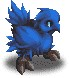
\includegraphics[width=0.23\columnwidth]{./art/chocobo/chocblue.jpg}}
{
	PV: & \hfill 15 & PM: & \hfill 25\\
	FOR: & \hfill 0 & DEF: & \hfill 0 \\
	MAG: & \hfill 2 & RES: & \hfill 1 \\
	AGI: & \hfill 2 & FOL: & \hfill 2 \\
}
{\accf{Bico}: 1d Dano \hfill \accf{Resistente:}\water}
{	
	\mspell{Água (Nível 1)}{6}{0r}{Único}{4u}{Cause 2d de dano de Água ao alvo.}{\accf{Nível 1}\water}	
	\mspell{Acumular (Nível 3)}{3}{0r}{Único}{5u}{O alvo ganha AuMAG por 3 rodadas.}{\accf{Level 3}\enmag}	
	\mspell{Águaga (Nível 6)}{14}{1r}{Único}{6u}{Cause 6d de dano de Água ao alvo.}{\accf{Nível 6}\water}	
	\mtech{Onda supersônica (Nível 9)}{18}{0r}{3u (frontal)}{Você}{Inimigos na área alvo sofrem 4d de dano e fazem um teste de DF~8, se falhar, ficam Mudos por 3 rodadas.}{\accf{Nível 9}\silence}
	\mpassive{Choco-nado}{Nade devagar através de qualquer rio ou mar sem corrente forte.}		
}
%
\clearpage
%
\ofmonster
{Chocobo Verde}{1}{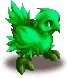
\includegraphics[width=0.23\columnwidth]{./art/chocobo/chocgreen.jpg}}
{
	PV: & \hfill 16 & PM: & \hfill 21\\
	FOR: & \hfill 0 & DEF: & \hfill 1 \\
	MAG: & \hfill 1 & RES: & \hfill 1 \\
	AGI: & \hfill 2 & FOL: & \hfill 2 \\
}
{\accf{Bico}: 1d Dano \hfill \accf{Imune:}\poison\blind\sleep}
{
	\mspell{Proteger (Nível 1)}{5}{0r}{Único}{5u}{O alvo ganha AuDEF por 3 rodadas.}{\accf{Nível 1}\enndef}
	\mspell{Regeneração (Nível 3)}{6}{0r}{Único}{5u}{O alvo ganha Regeneração por 3 rodadas.}{\accf{Nível 3}}	
	\mspell{Refletir (Nível 6)}{10}{0r}{Único}{3u}{O alvo ganha um escudo que reflete a próxima magia que o alveje de volta ao conjurador.}{\accf{Nível 6}}	
	\mspell{Vida-Cheia (Nível 9)}{24}{1r}{Único}{3u}{Remova o estado de KO do alvo e restaure o PV dele completamente.}{\accf{Nível 9}\ko}	
	\mpassive{Choco-socorros}{Enquanto não em combate, gaste 10 minutos para curar um aliado de um Estado de Efeito, exceto KO.}
}
%
\vfill
%
\ofmonster{Chocobo Branca}{1}{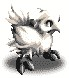
\includegraphics[width=0.23\columnwidth]{./art/chocobo/chocwhite.jpg}}
{
	PV: & \hfill 18 & PM: & \hfill 24\\
	FOR: & \hfill 1 & DEF: & \hfill 0 \\
	MAG: & \hfill 1 & RES: & \hfill 1 \\
	AGI: & \hfill 2 & FOL: & \hfill 3 \\
}
{\accf{Bico}: 1d Dano \hfill \accf{Resistente:}\holy}
{	
	\mspell{Acelerar (Nível 1)}{8}{0r}{Único}{3u}{O alvo fica Acelerado por 3 rodadas.}{\accf{Level 1}}
	\mspell{Vento brando (Nível 3)}{14}{0r}{4u (linha)}{Você}{Aliados na área alvo recuperam PV igual a metade de seu PV atual e são curados de todos os Estados Negativos, exceto KO.}{\accf{Nível 3}}
	\mspell{Recarregar (Nível 6)}{8}{1r}{3u}{Você}{Aliados dentro da área alvo, exceto você, recuperam 3d de PM.}{\accf{Nível 6}}
	\mspell{Sagrado (Nível 9)}{20}{2r}{Único}{7u}{Cause 6d+20 de dano Sagrado ao alvo.}{\accf{Nível 9}\holy}
	\mpassive{Choco-sentido}{Sinta a presença de monstros hostis a uma distância de até 200u.}		
}
%
\vfill
%
\ofquote{"Ela dirá quanto estiver pronta, então tire seus Chocobinhos da chuva até lá, tá?"}{Wakka}
%
\newpage
%
\ofmonster{Chocobo Preta}{1}{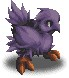
\includegraphics[width=0.23\columnwidth]{./art/chocobo/chocblack.jpg}}
{
	PV: & \hfill 19 & PM: & \hfill 23\\
	FOR: & \hfill 1 & DEF: & \hfill 1 \\
	MAG: & \hfill 1 & RES: & \hfill 0 \\
	AGI: & \hfill 2 & FOL: & \hfill 3 \\
}
{\accf{Bico}: 1d Dano \hfill \accf{Resistente:}\dark}
{
	\mspell{Gravidade (Nível 1)}{6}{0r}{Único}{3u}{O alvo sofre 2d de dano e só pode se mover metade de seu movimento no próximo turno.}{\accf{Nível 1}}
	\mspell{Petrificar (Nível 3)}{7}{1r}{Único}{5u}{O alvo faz um teste de DF~8 ou fica Imóvel por 3 rodadas.}{\accf{Nível 3}\immobile}
	\mspell{Imperil (Nível 6)}{10}{1r}{Único}{5u}{O alvo sofre ReDEF e ReRES por 3 rodadas.}{\accf{Nível 6}\dedef \deres}	
	\mspell{Última (Nível 9)}{25}{2r}{2u}{7u}{Cause 6d+35 de dano de Escuridão a todos os inimigos na área alvo.}{\accf{Nível 9}\dark}
	\mpassive{Choco-voo}{Voe até 50u acima do chão.}		
}
%
\vfill
%
\ofmonster{Chocobo Dourada}{1}{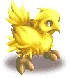
\includegraphics[width=0.23\columnwidth]{./art/chocobo/chocgold.jpg}}
{
	PV: & \hfill 25 & PM: & \hfill 35\\
	FOR: & \hfill 1 & DEF: & \hfill 1 \\
	MAG: & \hfill 1 & RES: & \hfill 1 \\
	AGI: & \hfill 3 & FOL: & \hfill 3 \\
}
{\accf{Bico}: 2d Dano \hfill \accf{Imune-a-tudo}}
{
	\mtech{Brilhar (Nível 1)}{5}{0r}{3u}{Vocês}{Inimigos na área alvo realizam um teste de DF~7 ou ficam Cegos por 2 rodadas.}{\accf{Nível 1}\blind}
	\mtech{Good Breath (Nível 3)}{8}{0r}{3u (frontal)}{Vocês}{Remova todos os Estados de Efeito, exceto KO, de todos os aliados na área.}{\accf{Nível 3}}	
	\mspell{Diaga (Nível 5)}{14}{1r}{Único}{6u}{Cause 6d de dano Sagrado ao alvo.}{\accf{Nível 5}\fire}
	\mspell{Curaja (Nível 7)}{20}{2r}{3u}{5u}{Aliados na área alvo recuperam 6d+15 de PV.}{\accf{Nível 7}}	
	\mtech{Choco-meteoro (Nível 8)}{27}{2r}{3u}{10u}{Todos na área alvo sofrem 6d+40 de dano.}{\accf{Nível 8}}	
	\mtech{Fênix final (Nível 10)}{30}{2r}{3u}{Vocês}{REmova KO de todos os aliados na área alvo e restaure o PV deles completamente.}{\accf{Nível 10}}	
	\mpassive{Choco-sentido}{Sinta a presença de monstros hostis a até 200u de distância.}		
	\mpassive{Choco-voo}{Voe até 50u acima do chão.}	
}
%
\clearpage